\section{Results}
\label{sec:results}
In this section we present the results of our simulation scenarios. The simulation reveals ...

\subsection{\Dc{} utilisation}
\Dc utilization markedly correlates with the number of potential service subscribers in network $N_{\ue}$. The effect is illustrated Figure \ref{fig:process}, which shows a strong growth of VM utilization when approaching maximum stable load at $N_{\ue}=800$, measured in the percentage of time it spends processing requests. Nevertheless, the process utilization starts to decay once we pass the number of stable subscribers, as more resources are now need to migrate differed users. Conversely, Figure \ref{fig:idle} shows how, as a result of increased parallel session residency, the proportion of time spent idle decreases dramatically.

\begin{figure}[tb]
	\centering
	%\includegraphics[height=0.175\paperheight]{diagram_overview.eps}
	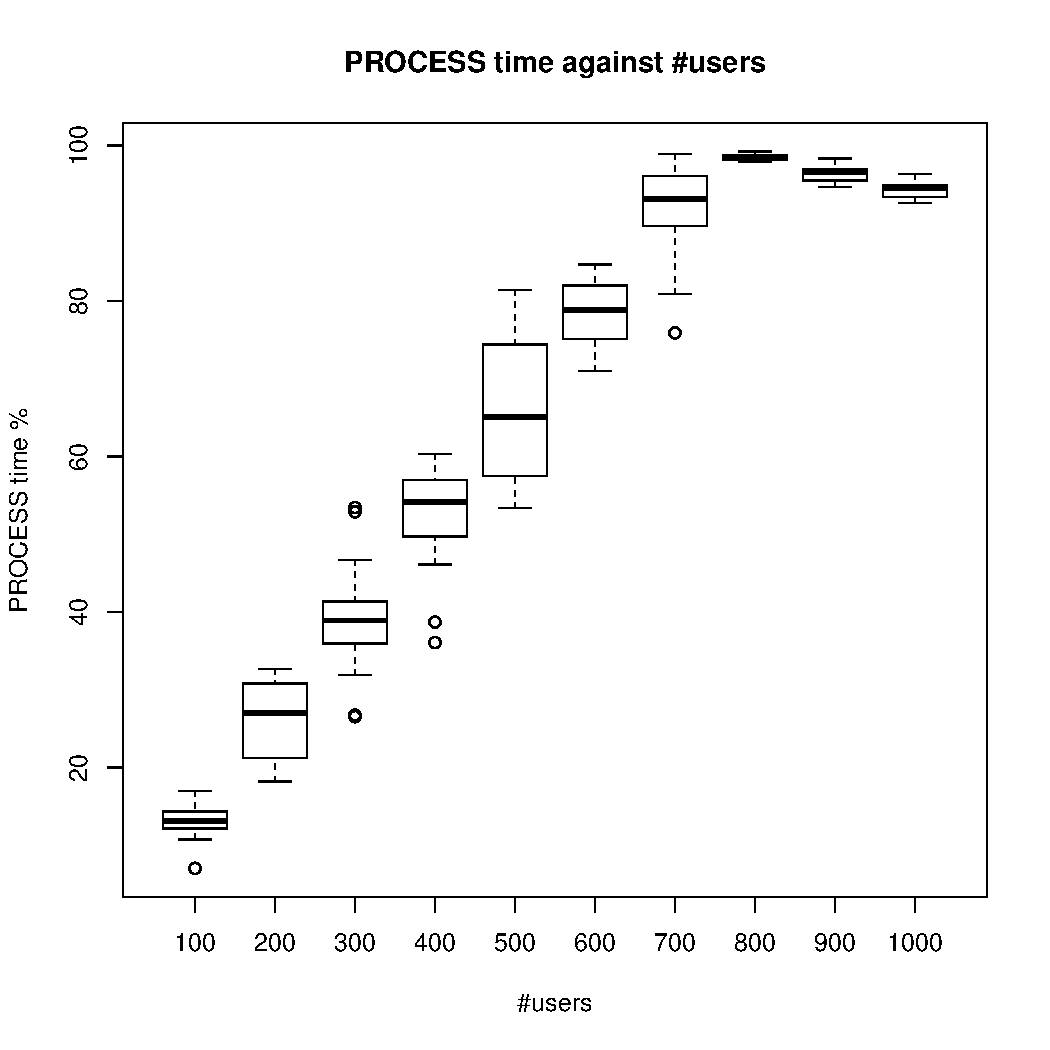
\includegraphics[width=\linewidth]{PROCESS.pdf} 
	\caption{Amount of time spent processing vs. the number of \ues in the entire network}
	\label{fig:process}
\end{figure}

\begin{figure}[tb]
	\centering
	%\includegraphics[height=0.175\paperheight]{diagram_overview.eps}
	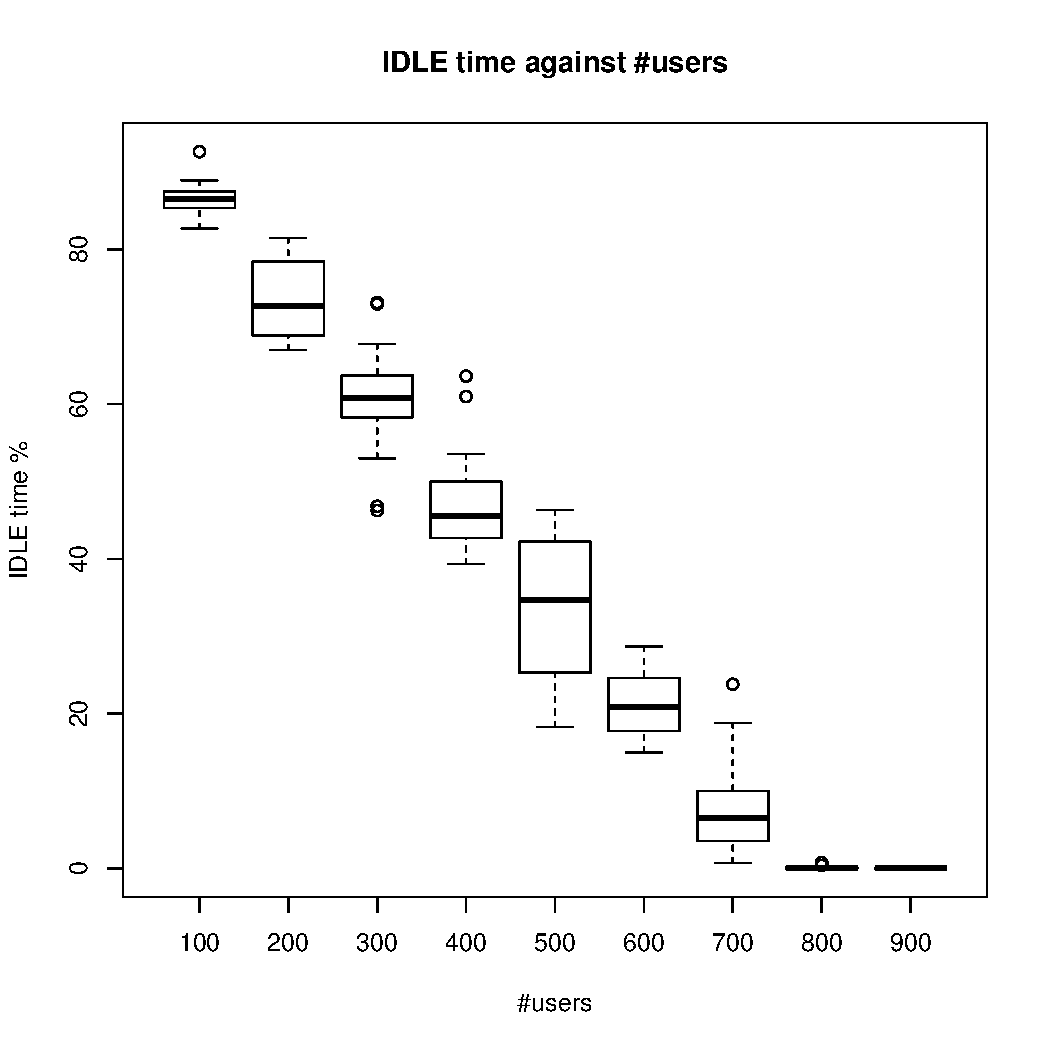
\includegraphics[width=\linewidth]{IDLE.pdf} 
	\caption{Amount of time spent in idle state vs. the number of \ues in the entire network}
	\label{fig:idle}
\end{figure}

Similarly, compounded by an increased likelihood of congestion in any given VM, the amount of requests needing to be migrated increases near exponentially with a growing number of subscribers $N_{\ue}$. Figure \ref{fig:transferring} illustrates the growth in the amount of time spent on migrating sessions.

\begin{figure}[tb]
	\centering
	%\includegraphics[height=0.175\paperheight]{diagram_overview.eps}
	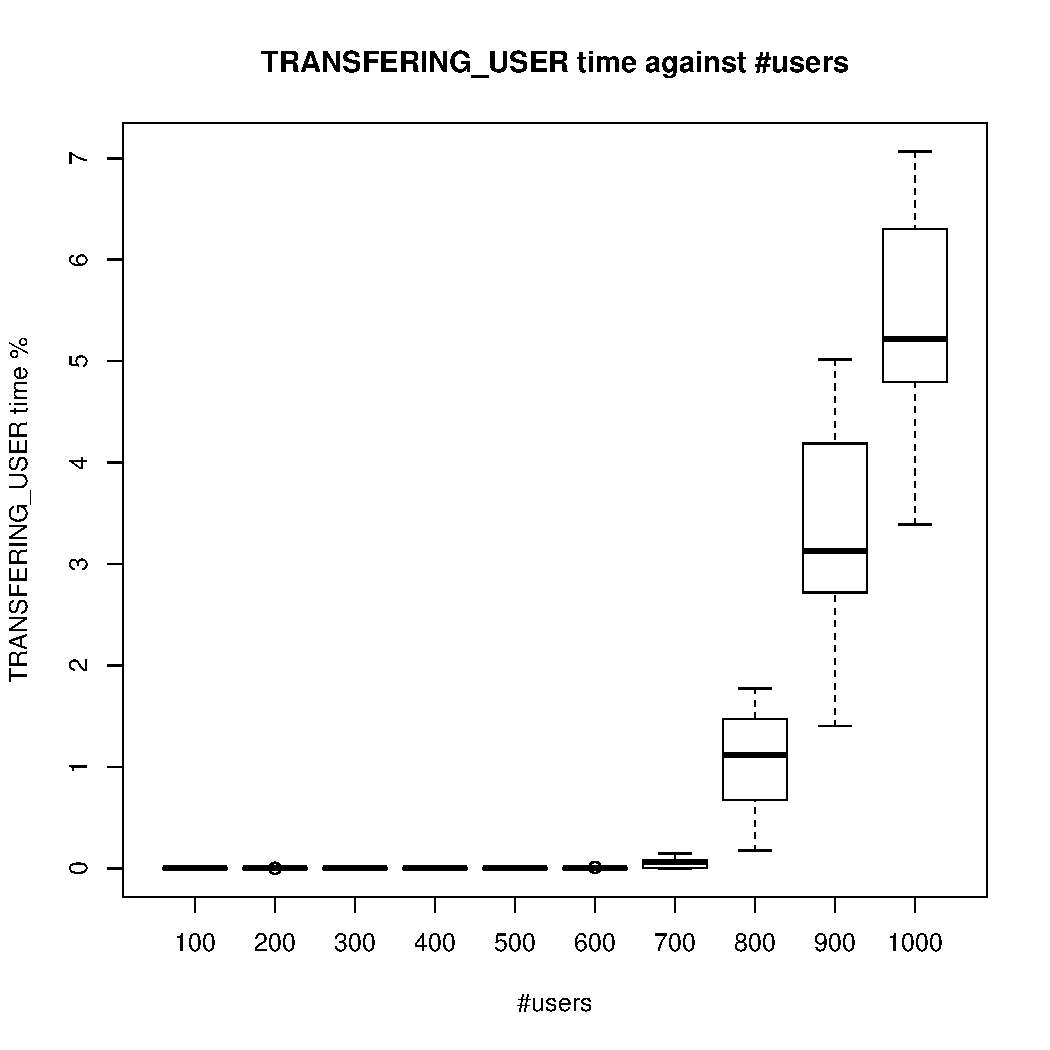
\includegraphics[width=\linewidth]{TRANSFERING_USER.pdf} 
	\caption{Amount of time spent transferring requests vs. the number of \ues in the entire network}
	\label{fig:transferring}
\end{figure}

\begin{figure}[tb]
	\centering
	%\includegraphics[height=0.175\paperheight]{diagram_overview.eps}
	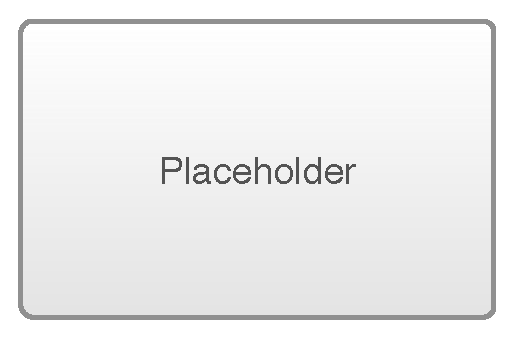
\includegraphics[width=\linewidth]{placeholder.eps} 
	\caption{Number of times a session is migrated vs. the number of \ues{} in the entire network}
	\label{fig:session_migration}
\end{figure}

\subsubsection{\Dc{} dispersion}

\subsection{Constrained \dc{} resources}

\subsection{Service performance}

\subsection{Properties of migration}
\subsubsection{Session completion grade per visited VM}

\subsection{Inter-\Dc{} communication}